\documentclass[letterpaper,11pt]{article}

\usepackage[margin=2.0cm]{geometry}
\usepackage{hyperref}
\usepackage{graphicx}

\title{Goto -- Milestone \#4 and final report\\Compiler design -- COMP 520}
\author{Jacob Errington \& Fr\'ed\'eric Lafrance}
\date{15 April 2016}

\begin{document}

\maketitle

\section{Introduction}
\label{sec:intro}

Goto is our compiler for GoLite, a subset of the Go language. It is written in Haskell and targets x86-64 assembly respecting the System V application binary interface (ABI) and C++. Our reasons for these choices, and indeed the choice of writing a compiler at all, are both philosophical and practical. From a philosophical perspective, compilers are one of the most general and powerful abstractions one can think of: they are at the core a transformation from one structured data type to another. Compiler design is at the intersection of the theory of computation, algorithm design, programming languages and engineering. Furthermore, the techniques and material learned while building a compiler apply to a wide range of problems. It would thus be foolish to not take this opportunity to learn as much as we can on all the phases of compiler design.

On a more practical perspective, it is important to us to compile to a widely-used platform so that our code can run on as many machines as possible. This relates to the primary goal of compilers, which is to enable programmers to use abstractions and free themselves from minute hardware details in order to multiply the effect they can have on the world. 

Finally, on a more personal level, we enjoy challenges and the satisfaction of completing a large project such as this one is not be underestimated. Steve Yegge \href{http://steve-yegge.blogspot.ca/2007/06/rich-programmer-food.html}{said} that a compiler design class \emph{``makes you a Real Programmer and puts hair on your chest, regardless of gender or chest-hair preference.''} We tend to agree with this sentiment.

This report is organized as follows. Section \ref{sec:tech} presents the technological choices we made in the design of our compiler. Section \ref{sec:arch} explains our consequent architectural choices and decisions. Team organization and task listings are presented in section \ref{sec:org}. In section \ref{sec:ph}, we explain in technical detail the phases of our compiler, from GoLite to assembly. This is followed by example output at all phases in section \ref{sec:eg}. Finally, we provide a recap and potential avenues for future work.

\section{Technology choices}
\label{sec:tech}

Functional programming languages are entering the mainstream as developers begin to understand how to take advantage of expressive type systems and powerful abstractions to build bug-free software with minimal effort. Even traditionally non-functional languages such as Java and C++ now have first-class functional features, while on the other end of the spectrum languages like Scala, Clojure and F\# are gaining rapid adoption. Among those, the Haskell programming language strikes a balance between being practical thanks to its high-quality tooling and having an expressive type system allowing us to devise extremely useful generalizations which will be detailed in section \ref{sec:arch}.

As for the target language, our decision to generate x86-64 assembly has simple motivations: x86 is the most ubiquitous general-purpose processor architecture in use today. Therefore, it is only natural that we decide to target it. Further, targeting a low-level representation forces us to write a compiler that has all the necessary features to go as low as we want, while still easily allowing us to target a higher-level language if we so desire.

Because of time constraints, we only generate assembly compatible with the System V ABI, which is in use on Unix-like systems. Further, we do not generate our own ELF file, but rather an assembly source file which we then assemble using the well-known YASM.

This choice of targeting x86-64 also means that we need a runtime which can be tied easily to our generated code. The C language is exactly what we need in this case, given its simplicity, ubiquity and interoperability.

\section{Architectural choices}
\label{sec:arch}

As mentioned before, our choice of Haskell as the implementation language means that we have at our disposal many powerful abstractions to write a clean, easily extensible compiler.

The first building-block we make use of is perhaps the most simple: the algebraic data type. We use various abstract syntax trees throughout our compiler. Thanks to type parameters, we are able to specify only the \emph{shape} of a tree, while the actual \emph{data} it contains is left abstract. This gives us a very simple yet very flexible way to annotate our syntax tree, by specifying different kinds of data. This way, the same base data type is re-used (for example) to construct test cases (no annotations), perform the initial parsing phase (source position annotations) and typecheck (GoLite type annotations).

Secondly, this parametrization also allows us to specify complete syntax trees as fixed-point operators over our AST types. Essentially, the fixed-point represents the fact that the children of statements and expressions are other statements and expressions. This enables us to use a generalized bottom-up fold over our AST. The name for this operation is \emph{catamorphism}. Throughout our project, we use catamorphisms basically any time a complete traversal of a syntax tree is required: weeding, typechecking, simplification and compilation. This completely general fold frees us of the worries of how to walk the tree so that we can focus on the actual transformations instead.

As we are generating assembly code, it is much simpler for us to go through an intermediate representation. We therefore have such a language, called Vigil, and we also have a pass converting our GoLite AST into a Vigil AST. This Vigil AST is then the one that is converted to assembly.

We have two different representations of assembly: one with virtual registers and one with only hardware registers. This allows us to separate concerns between generating valid assembly code from a Vigil AST, and carrying out register allocation. In this, we follow a well-known tradition in compilers. GCC was our inspiration for many decisions at this stage, including the Vigil grammar and some idioms related to virtual registers (we did not, however, come up with our own Register Transfer Language).

The two representations of assembly, being very similar, are of course abstracted to a single data type that contains an abstract \texttt{register} parameter. Another general abstraction that we make use of here is that of the free monad. Briefly, a free monad allows us to build data representations in a manner that is agnostic to the way we will use (\emph{interpret}) it later. Our generated assembly code is still a functor fixed point (this time over a list rather than a tree), but thanks to the free monad we get the power of do notation and chaining actions together for free. This means for example that the code computing register lifetimes or transforming the virtual assembly to regular assembly is completely straightforward and reads perfectly sequentially.

Finally, sometimes the cleanest way to represent a computation is by using mutable state. This is the case in our register allocator, which maintains shared memory cells that represent the allocation state of a given virtual register. When a decision is made concerning a particular register, its state is updated, immediately affecting all the other registers. This gives us a working register allocator in barely over 200 lines of code.

To summarize, our guiding principles when building Goto were to abstract away as many details on the shape of the data as possible, to allow us to write general code to operate on all the different data representations we need. A perfunctory count suggests that a compiled program goes through six of those representations before reaching the executable state. By using the expressiveness of Haskell's type system to our advantage, we make the transitions between these various stages as simple as possible.

\section{Team organization}
\label{sec:org}

As a two-person team, the communication overhead was greatly reduced and many tasks divided themselves naturally, which almost compensated for the fact that we were in fact two and not three. Table \ref{tab:dol} presents an overview of the tasks accomplished by the team members for every phase of the project. As expected, design decisions, documentation and bug-fixing were a joint endeavor.

\begin{table}
	\begin{tabular}{|l|p{15em}|p{15em}|}
	\hline
	& \textbf{Jacob} & \textbf{Fr\'ed\'eric} \\
	\hline
	Scan~/ parse & AST definition, annotation strategy, expression parser, semicolon management, pretty-printer. & Lexers, statement~/ declaration~/ top-level parsers, annotation stripping strategy, test generators, manual test cases. \\
	\hline
	Weed~/ typecheck & Scoping rules, typechecking of statements and many expressions, type pretty-printing & Weeder, typechecking of binary operators~/ unary operators~/ built-ins, symbol table dumping, integration tests \\
	\hline
	Simplify & Global identifier management, identifier renaming, IR type system & IR grammar, AST-to-IR conversion \\
	\hline
	Compile & Compilation of IR to virtual assembly, pretty-printing of hardware and virtual assembly, C++ code generator & Register allocation, virtual-to-hardware translation, C runtime \\
	\hline 
	\end{tabular}
	\caption{Division of labor in team 04}
	\label{tab:dol}
\end{table}

\section{Phases}
\label{sec:ph}

This section deals with the actual guts of the compiler and is as such much more technical than section \ref{sec:arch}. As one would expect, we present our compiler sequentially, going phase by phase from textual GoLite input to assembly file output.

\subsection{GoLite AST generation}
\label{sec:ph_parse}
The Haskell Parsec library brought the idea of monadic parser combinators into the mainstream and essentially pioneered this kind of parsing as an alternative to the more traditional lexer/parser generators. Rather than describe the grammar of the language to parse in a domain-specific language such as Sable, Parsec lets the programmer describe a parser using intuitive \emph{embedded} combinators that benefit from the full strength of Haskell. We are using a fork of Parsec called Megaparsec that includes even more advanced combinators that greatly facilitate the writing of certain kinds of common parsers (notably basic whitespace and token handling, as well as sequences of parsers).

We decided to write idiomatic Parsec code by having small, highly-combinable parsing functions (which we call parsers for short). Those were then put together to form the more complex statement, declaration and expression parsers. It is important to note here that the distinction between lexing and parsing is blurred here: our most basic combinators are still called ``parsers'', but perform very simple tasks such as consuming whitespace, or words, or various operator symbols. Parsec handles infinite lookahead and easy backtracking (in fact, some would say \emph{too} easy), which means our grammar is very straightforwardly specified as the code that parses a GoLite source file.

In order to handle semicolon insertion properly, we decided to use a State/Exception monad (the \texttt{Semi} monad) and write various combinators to make our parsers work with this monad. The benefits of this approach are twofold. First, we do not have to modify the underlying source file, therefore preserving position information for error messages. Second, we can write our parsers in a mostly semicolon-agnostic way, and combine them with the \texttt{Semi} monad whenever actual handling is required. This was useful to handle some tricky cases, such as simple statements always requiring semicolons except in the post-iteration position of a for loop, or blocks always requiring semicolons except in the case of an if/else statement, or even comments triggering semicolon insertion.

The result of this first pass is a source-annotated GoLite syntax tree. These source annotations are used in subsequent phases for error reporting. The first place where this occurs is the weeding phase, which deals with rejecting various classes of invalid programs. Since we have essentially the most powerful grammar possible (executable code), it is mostly a matter of convenience as to what ends up in the weeder checks vs. earlier parser checks. The general rule we used was that if it involved checking the state of more than one tree node at a time, it should go in the weeder. This divide is quite natural. For example, lvalue checks occur at the parser level, since they can be done entirely by looking at a parsed expression when building an assignment node. On the other hand, function termination analysis involves going down over potentially several paths of the tree to check that all of them end in a terminating statement (whose definition is actually quite complex and includes \href{https://golang.org/ref/spec#Terminating_statements}{eight different cases} in Go). Therefore, these checks occur in the weeder. The weeder is a catamorphism of the tree into a unit value; indeed, we are not interested in transforming the tree into anything, but simply in the state (i.e. potentially thrown errors) of the computation.

\subsection{Symbols and typechecking}
\label{sec:ph_type}

The typechecking phase is another stateful tree traversal, but which this time has a final value: a type-and-source-annotated syntax tree. In this phase, we build our symbol table and typecheck the program simultaneously, which can be done thanks to the fact that GoLite is quite simple and does not support mutual scopes (i.e. declarations are ordered). The symbol table is a standard cactus stack (a stack of dictionaries, where the dictionaries are standard-issue Haskell containers implemented as binary search trees) which we keep in the state of the traversal. We have at our disposal several combinators, which allow us to transform any typechecking action by introducing a new scope around it, or performing symbol declarations. As we progress through the typechecking of the tree, we add more information to this symbol table, which is looked up whenever we need to typecheck expressions containing some kind of identifier.

We have a fixed-point datatype representing a GoLite type. In addition to the standard types, we keep track of type aliases (which have decidedly confusing typechecking rules), function types, as well as a host of properties which indicate which types can be used to perform which operations (e.g. is a type arithmetic, logical, printable, and so on).

Typechecking itself is a fairly routine tree traversal. A lot of very specific code had to be written to handle corner cases, but the general pattern is predictable. One interesting aspect of this catamorphism is the transformation of identifiers from simple strings to global identifiers. We take every single user-supplied identifier into a data type called a global ID, which contains a globally unique identifier, as well as the type of the original identifier. This means that we can quite simply throw away the symbol table with its scoping information once we are done: identifiers naturally get different names given their scopes, and now carry their types. We are able to so easily replace all identifiers because our AST data type abstracts away the data it contains, as we explained in section \ref{sec:arch}.


\subsection{Simplification to Vigil}
\label{sec:ph_simpl}

Targeting x86-64 directly from GoLite is fraught with peril. This is why we have an intermediate representation called Vigil which is considerably simpler than GoLite and allows us to use a template-based approach to code generation. Vigil is a ``language'' in its own right, although its programs are not valid GoLite anymore and thus cannot be compiled by anything. However, it is quite simple to pretty-print them.

The Vigil syntax is very nearly the same as \href{https://web.archive.org/web/20040308142632/http://www-acaps.cs.mcgill.ca/info/McCAT/public/intermediate.html#SIMPLE}{SIMPLE} with a few minor modifications for the GoLite use case. Much of the simplification process involves transforming expressions into a three-address form by inserting temporary variables strategically. At the statement level, some statements are entirely discarded (e.g. empty statements and type declarations), flattened (blocks), or moved around (e.g. declarations are moved to the top of a function declaration, initializer statements of if blocks are moved just before them, additional statements for temporaries are inserted, and so on).

Despite being called ``simplification'', the process of taking a source-and-type-annotated GoLite AST into a type-annotated Vigil AST is actually not that straightforward. The main issue is that expressions in Vigil are in three-address form, which means that complex expressions must be broken down and appropriate temporaries generated. The catamorphism over GoLite expressions thus returns a stack of ``expression results'', where the top of the stack is the final computation in the expression (the one which actually represents a value), while the lower elements of the stack represent temporaries. As the expression is simplified further and further, this stack is percolated up the tree, with every node potentially adding its own temporaries. This process is further confounded by the presence of short-circuiting operations: an expression like \texttt{a \&\& b} is really translated as an if statement which first evaluates \texttt{a}, and then evaluates \texttt{b} only if \texttt{a} is true. Since while we are simplifying an expression we do not output any sort of statements, we just keep track of all these intermediate results for later use.

It is in fact at the moment of transforming statements that we take these stacks of expression results into actual statements (a process which we call ``realization''). A common pattern is as follows: a given statement contains an expression. We first simplify and realize the expression, which gives us a list of statements and a final result. Depending on how we choose to realize the expression, this final result may be a full-fledged expression (for use in assignements, for example), a reference (which can occur in some simple statements) or a value (which is generally restricted to contexts where we specifically need a variable or a literal, such as in calls). The realization process generates all the statements to put something useful in this result, which is then used in the simplified version of the statement. The realization operation also modifies the state of the monadic computation by recording which temporary variables have been declared. Then, once the statements have been simplified, the function that contains them is extended with these new variable declarations. A similar process occurs for global variables, although in this case all initialization statements are moved to an \texttt{init} function which we synthesize.

Once this process is complete, we have a type-annotated Vigil syntax tree. As much as we'd like to get rid of the type annotations, they are actually necessary later on to generate the proper machine code so we need to keep them.

\subsection{Assembly generation}
\label{sec:ph_gen}

Assembly generation is itself a multi-pass phase. We have the following transformations.

\subsubsection{Vigil to virtual assembly}
\label{sec:vasm}

We transform our Vigil AST into a free monad representation of the assembly code. We use an assembly data type that abstracts over its operands (which are virtual at this stage) and label types. The compilation is template-based: every Vigil statement and expression is matched to a specific template, which is output as a value in the free monad. This assembly contains virtual registers. There is normally one virtual register per variable. Some instructions are output with fixed registers, meaning that they must access a specific register. This occurs for example in calls: we need to respect the System V ABI which specifies, amongst other things, which registers are used to pass which parameters.

Special handling is done for managed data types (i.e. arrays, slices and structs). The runtime has several functions dedicated to using them, which means that they are treated mostly as opaque integers (pointers) from the assembly point of view.

A virtual register also carries information about the way it should be accessed, namely its size (low byte, high byte, word, double word, quad word) and kind (integer or floating-point). This information is used in the forthcoming passes.

The generated virtual assembly also contains some pseudoinstructions at interesting program points. Notably, we have one such instruction at each function entry and exit, so as to later allocate/deallocate the proper amount of space on the stack. We also have other save and restore pseudo-instructions around calls to save the registers which are considered to be scratch and might thus be modified by the called function.

\subsubsection{Lifetime analysis}

We run an interpreter on the virtual assembly free monad whose job is to compute the lifetimes of all registers. We use an extremely basic register allocation scheme which only admits simple lifetimes without holes. Therefore, every virtual register is live from its first to last reference. We do only the most basic control flow analysis: in the case of a jump backwards (such as in a loop for example), the lifetime of virtual registers that are live between the jump point and target are extended to fill the entire area that was jumped over. This ensures that the lifetimes of variables are appropriate in loops.

The result of this interpretation of the free monad is a map of virtual registers to lifetimes. This data is directly used in the next two sub-phases of code generation.

\subsubsection{Register allocation}

Because we do essentially no data-flow analysis, we employ a very simple register allocation strategy, which is not especially close to optimal but has the advantage of being easy to understand and implement, as well as fast to run. The strategy in question is just linear allocation. We order the virtual registers by their lifetimes and allocate hardware registers on a first-come, first-serve basis based on the kind of the register. In the interest of simplicity, we currently ignore sizes and always allocate a full quad-word hardware register to a given virtual register.

To perform the actual allocation, we also compute for every virtual register what are the other virtual registers that have overlapping lifetimes. This is the part of the compiler where we use state in the most direct manner: by declaring for every virtual register a memory cell (Haskell's version of a pointer, essentially) which contains its allocated hardware location (a hardware location being either a hardware register or a ``memory location'', the details of which are undefined at this point). This way, as we walk down the priority queue of lifetime intervals, allocating a register is immediately propagated to the conflict lists that we keep track of.

For every virtual register, the following very simple decision procedure is run. We first check if any of the hardware registers with the suitable access kind are available. If yes, we assign one of them to the virtual register. If no, we have to spill something to a memory location. The heuristic we choose is to spill the virtual register which lives the furthest in the future (which can be the virtual register we're trying to allocate something for).

There are two registers which we never allocate: \texttt{rax} and \texttt{xmm0}. The reason for this is twofold. First, those registers are used for return values, so computing their lifetime could be difficult (given a series of calls, it's not clear which one of them returned the value into \texttt{rax} that we want to use now). Second, we need a scratch register in cases where an instruction involving two virtual registers sees both of those registers spilled. Indeed, in x86, memory~/ memory operations are disallowed. We thus need to guarantee that a register will always be available to convert those to a pair of instructions, one register~/ memory and the other memory~/ register.

To conclude, at the end of the register allocation process, we are left with a mapping from virtual registers to hardware locations. This is exactly what we need to convert our virtual assembly code.

\subsubsection{Virtual to hardware assembly}

From our virtual register~/ hardware location mapping, we first compute a few useful values, such as the total amount spilled and the safe registers we used (and that we will have to save~/ restore at function entry~/ exit). We then do another interpretation of our virtual assembly free monad. This time, the result is another monad containing the hardware assembly.

The mapping is very routine and mostly involves translating the instruction operands with the help of the virtual-to-hardware map generated by our register allocator. As explained in section \ref{sec:vasm}, this is where we replace our various pseudoinstructions with actual code to conform to the ABI, manage spills and generate labels.

\subsection{Hardware assembly to executable file}

Given our hardware assembly, we can simply pretty-print it to a textual representation that YASM will accept. This involves generating some required boilerplate to interface with our runtime: our assembly file exports the functions \texttt{gocode\_main} and \texttt{gocode\_init} which are called by the runtime, and imports all the runtime functions. The runtime is a monolithic C library that defines various functions for creating and using managed objects, and is not particularly interesting in and of itself.

This assembly file is then passed through YASM, which produces an object file. We link that against our runtime, which contains a main function that calls \texttt{init} then \texttt{gocode\_main}, to get an executable.

\subsection{C++ code generation}

At the last minute, in a last-ditch effort to get output that would be able to run at least our example programs from the last milestone, we implemented a C++ code generator. This code generator translates the typechecked GoLite AST directly into a C++ string.

The traversal of the GoLite AST is done by a catamorphism as usual, but with some special considerations for the names of types that occur in the source code. Since we originally planned on targeting only x86, we paid little consideration to type declarations, since we recorded the types of variables \emph{in the variables themselves}. However, in order to generate correct C++ code, we must of course declare the structs that are used by the program.

The guiding principle of the traversal is that we \emph{delay} deciding how to name types until the traversal is complete. This is achieved by having the traversal compute a \emph{function} that takes a map from \texttt{Type}s to strings at the same time as the map is built up. The reason we have to use this map is to guarantee that the same name is given to two instances of the same type (i.e. two anonymous structs with the same fields in the same order are given the same type name in the C++ code.) Once the traversal is complete and the both the map and the function are built up, we call the function with the map in order to produce the final output string.

The implementation of the C++ runtime was very simple since we chose to implement Go slices with STL vectors, Go arrays as STL arrays, and Go strings as STL strings. All of these data types support a \texttt{size} method, for instance, so it was trivial to define a \texttt{len} template function in the runtime that simply invokes the \texttt{size} method of the object that it is given without concern for the exact type of the object.

\subsection{Phase diagram}
\begin{figure}[ht]
\begin{center}
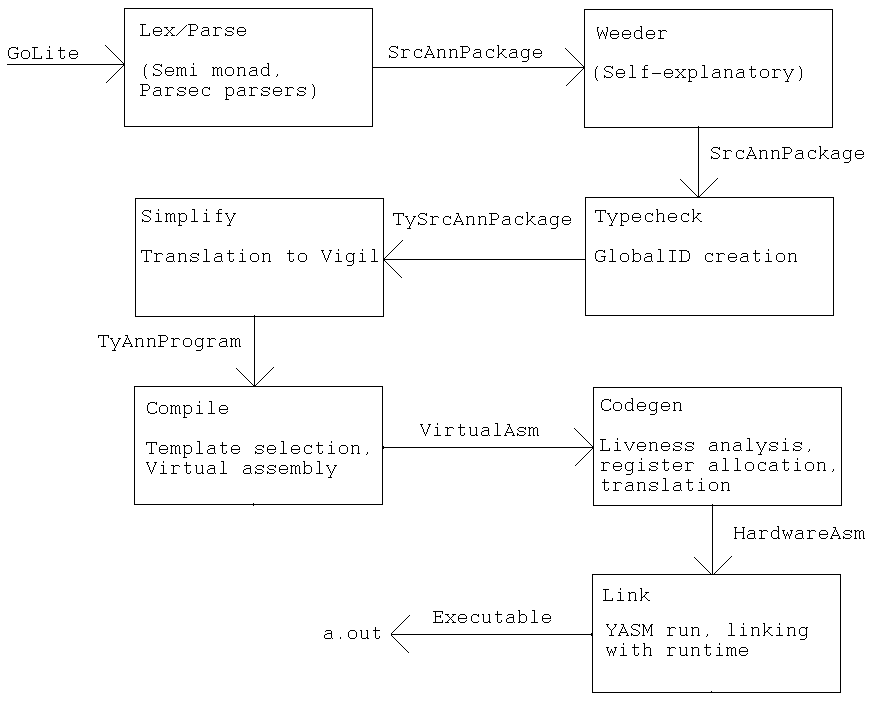
\includegraphics[width=.6\textwidth]{diagram.png}
\end{center}
\caption{Phases of the goto compiler to generate x86 code}
\end{figure}

\section{Example output}
\label{sec:eg}
We show a program as it goes through the main phases of our compiler.
\subsection{GoLite}
This program is very simple, but quickly grows as it reaches the assembly stage.
\begin{verbatim}
package main
func main() {
    if z:= true; z {
        println(z)
    }
}
\end{verbatim}

\subsection{Typed AST}
The types of all sub-expressions are printed as comments next to the expressions. Also notice the identifier renaming to guarantee uniqueness, allowing us to throw away scoping information.
\begin{verbatim}
package main
func gocode_main_14 () {
    if gocode_z_15 := gocode_true_5 /* bool (untyped) */ gocode_z_15 /* bool */ {
        print(gocode_z_15 /* bool */, ""\n"" /* string (untyped) */)
    }
}
\end{verbatim}
\subsection{Vigil AST}
Note the simplification process added the synthetic init function, and moved the initializer statement out of the if statement. The empty double brackets represent places where extra temporaries would be declared if they were needed.
\begin{verbatim}
var strlit17_17

func init_-1 {
    [[]]
    var gocode_z_15
    strlit17_17 = _from_cstr#([strlit17data_18])
}

func gocode_main_14 {
    [[]]
    var gocode_z_15
    gocode_z_15 = 1
    if gocode_z_15 {
        print (gocode_z_15, strlit17_17)
    }
}
\end{verbatim}
\subsection{Virtual assembly}
Note that here the variable \texttt{z} was given the virtual register \texttt{vi0}. Other registers seen are fixed, which means that the ABI requires us to use those registers specifically.
\begin{verbatim}
init:
    push rbp
    mov rbp , rsp
    mov rdi , QWORD strlit17data
    call _from_cstr
    mov vi1 , rax
    mov QWORD [strlit17 + 0] , vi1
    mov rsp , rbp
    pop rbp
    ret
gocode_main:
    push rbp
    mov rbp , rsp
    mov vi0 , 1
    test vi0 , vi0
    je l0
    mov rdi , 1
    mov rsi , vi0
    call _goprint
    mov rdi , 6
    mov rsi , QWORD [strlit17 + 0]
    call _goprint
    l0:
    mov rsp , rbp
    pop rbp
    ret
\end{verbatim}
\subsection{Hardware assembly}
This is output that YASM can assemble, so it contains the necessary extern/global definitions and divides the code into proper sections. Also note that no more virtual registers are present. Showing an example which triggers a spill would be unwieldy because of the extra amount of registers in x86-64.
\begin{verbatim}
BITS64
default rel
extern _goprint,  _from_cstr,  _index_slice,  _index_array,  _slice_slice,
   _slice_array,  _golen_slice,  _golen_array,  _goappend_slice,
   _concat_strings,  _gocopy,  _gocap,  _gopanic,  _gomake,  _deepcopy_struct,
   _deepcopy_array,  _shallowcopy_slice,  _new_array,  _new_slice,  _new_struct
global _init, _gocode_main
section .data
    strlit17data: db 10,  0
section .bss
    strlit17: resb 8
section .text
    _init:
        push rbp
        mov rbp , rsp
        sub rsp , 0
        mov rdi , QWORD strlit17data
        call _from_cstr
        mov rbx , rax
        mov QWORD [strlit17 + 0] , rbx
        add rsp , 0
        mov rsp , rbp
        pop rbp
        ret
    _gocode_main:
        push rbp
        mov rbp , rsp
        sub rsp , 0
        mov rbx , 1
        test rbx , rbx
        je l4
        push rdi
        sub rsp , 8
        mov rdi , 1
        mov rsi , rbx
        call _goprint
        add rsp , 8
        pop rdi
        push rsi
        sub rsp , 8
        mov rdi , 6
        mov rsi , QWORD [strlit17 + 0]
        call _goprint
        add rsp , 8
        pop rsi
        l4:
        add rsp , 0
        mov rsp , rbp
        pop rbp
        ret
\end{verbatim}

\subsection{C++ code generator output}
The output of our C++ code generator is extremely messy, given that it was cobbled together at the last minute. The extraneous typedef is the result of Go allowing complex types to be used anonymously. In particular, a struct can be used as the return value of a function without the struct previously being given a name with the `type` construct. Rather than introduce typedefs for anonymous structs as a special case, we simply create typedefs very liberally for pretty much every type encountered in the program.

\begin{verbatim}
// main
#include <iostream>
#include <memory>
#include <array>
#include <vector>
#include <string>
#include "goto.hpp"
using namespace std;
typedef bool type1;
bool _gocode_true = true;
bool _gocode_false = false;
void _gocode_main()
{
    {
        type1 _gocode_z = _gocode_true;
        if (_gocode_z)
        {
            cout << boolalpha << _gocode_z << "\n";
        }
    };
}
int main() { _gocode_main(); }
\end{verbatim}
\section{Conclusion and future work}

In terms of achieving the goal of learning as much as we could about compilers, we probably have done the most complete survey of the different phases of compiling that we could possibly have done in this amount of time. We used very few domain-specific helper libraries (Megaparsec being the main one) and went all the way to x86 generation, which gave us exposure to intermediate representations, register allocation and other considerations about instructions. We also learned a great deal about language interop at this lowest of levels. Overall, we think we learned that x86-64 assembly and the System V ABI are incredibly difficult to target, which explains the incompleteness of our native code generator. We both now have even more respect and admiration for the engineers who have built today's amazing compilers which until now we have taken for granted.

There are however several aspects which we had to cut or scale back in order to finish. We did not end up generating our own ELF file; in hindsight, this would have given us massive street cred but would also have been a relatively pointless exercise seeing as knowledge the intricacies of the file format is not an especially transferable skill. We also had a much simpler register allocator than originally anticipated. This is mainly because we did not properly research the topic beforehand and did not realize that we would have to do dataflow analysis for anything but the simplest register allocator, which would have taken another milestone by itself.

In terms of future work, we are therefore definitely interested in revisiting the post-typecheck phases. Some points that we consider are:
\begin{itemize}
    \item Getting the x86 code generator to fully work.
    \item Use the virtual assembly together with the Vigil representation to construct a basic-block graph of the program, to perform actual liveness analysis and allow us to do better register allocation;
    \item Implement mid-level optimizations at the Vigil stage (e.g. common subexpression simplification, function call inlining, loop invariant hoisting) and peephole optimizations at the hardware assembly stage (e.g. redundant \texttt{mov} elimination, lifetime merging)
    \item Extend our runtime to support garbage collection.
\end{itemize}

Of course, all these are fairly large tasks which could take a long time to finish. In the end though, the exercise of writing a compiler in Haskell targeting assembly exposed us to a great deal of general and powerful concepts and strategies that apply not only to compilation, but also to the treatment and transformation of any form of structured data. That is perhaps the most unique and important aspect of this project.

\section{Acknowledgements}
We acknowledge Brendan Gordon for moral support and bringing us coffee. We would also like to thank Vincent Foley-Bourgon for his excellent reference compiler and assistance throughout the project. Finally, we wish to thank Ken Thompson and Rob Pike for giving us a challenging language to work with.

\section{References}

\begin{itemize}
\item \href{https://golang.org/ref/spec}{The Go specification}
\item \href{http://www.sable.mcgill.ca/~hendren/520/2016/assignments/syntax.pdf}{The GoLite syntax specification}
\item \href {http://www.sable.mcgill.ca/~hendren/520/2016/assignments/typechecker.pdf}{The GoLite typecheck specification}
\item \href{https://play.golang.org/}{The Go playground}
\item The \href{http://wiki.osdev.org/System_V_ABI}{System V ABI page} at osdev.org
\item \href{http://www.x86-64.org/documentation/abi.pdf}{System V Application Binary Interface}
\item The documentation and source code of the following Haskell packages:
	\begin{itemize}
	\item \href{https://hackage.haskell.org/package/megaparsec-4.3.0}{Megaparsec} (main parser library)
	\item \href{https://hackage.haskell.org/package/hspec}{hspec} (unit test library) and the \href{http://hspec.github.io/}{associated manual}
	\item \href{https://hackage.haskell.org/package/QuickCheck-2.8.2}{QuickCheck} (test-case generator library) and the \href{http://www.cse.chalmers.se/~rjmh/QuickCheck/manual.html}{associated manual}
	\item \href{http://hackage.haskell.org/package/pretty-1.1.2.0/docs/Text-PrettyPrint-HughesPJ.html}{PrettyPrint.HughesPJ}, whose structure we used extensively in all our pretty-printing code.
	\end{itemize}
\item The following articles on building and working with generalized annotated syntax trees using functor fixed points and catamorphisms:
	\begin{itemize}
	\item \href{http://martijn.van.steenbergen.nl/journal/2010/06/24/generically-adding-position-information-to-a-datatype/}{\textit{Generically adding position information to a datatype}} and the associated \href{http://martijn.van.steenbergen.nl/projects/Selections.pdf}{thesis}
	\item \href{http://blog.plover.com/prog/springschool95-2.html}{\texttt{data Mu f = In (f (Mu f))}}
	\item \href{https://www.schoolofhaskell.com/user/edwardk/recursion-schemes/catamorphisms}{\textit{Catamorphisms}}
	\item \href{http://comonad.com/reader/2009/incremental-folds/}{\textit{Reflecting on incremental folds}}
	\end{itemize}
\item The following pages for inspiration on Vigil:
	\begin{itemize}
	\item \href{https://web.archive.org/web/20040812030043/www-acaps.cs.mcgill.ca/info/McCAT/McCAT.html}{McCat compiler}, for the SIMPLE grammar.
	\item The \href{https://gcc.gnu.org/onlinedocs/gccint/GIMPLE.html#GIMPLE}{GIMPLE} syntax.
	\end{itemize}
\item These items on register allocation:
	\begin{itemize}
	\item \href{https://hackage.haskell.org/package/linearscan}{\texttt{linearscan}}, a Haskell package for register allocation that we decided not to use since it does not appear to be adapted to our use case (can't differentiate between types of registers, for instance).
	\item \href{http://www.christianwimmer.at/Publications/Wimmer04a/Wimmer04a.pdf}{\emph{Linear Scan Register Allocation
	for the Java HotSpot Client Compiler}}, Wimmer 2004.
	\end{itemize}
 
\item Miscellaneous:
	\begin{itemize}
	\item \href{http://blog.ezyang.com/2014/05/parsec-try-a-or-b-considered-harmful/}{Parsec: \texttt{try a <|> b} considered harmful} (in order to generate better-quality error messages).
	\item
	\href{http://book.realworldhaskell.org/read}{Real-world Haskell}, which Fred bought a hardcopy of a while ago and needed a reason to read.
	\end{itemize}
\end{itemize}

\end{document}
